%% ============================================================
\section{Experiments}\label{sec:experiments}
%% ============================================================

We ask how composition scales with sampling (RQ1), how much compositional
inference and training improve verification (RQ2), how \sam{} compares with
specialized tools (RQ3), how RL reshapes compositional exploration before and
after SFT (RQ4),
and how credit assignment affects compositional exploration under RL (RQ5).

\subsection{Experimental Setup}
\label{sec:exp:setup}

\tightparagraph{Data and judge.}
Training data comprise 4,992 RL records and 33,346 SFT records (31,865
distinct sources) of target-masked scalar-integer single-loop programs;
Appendix~\ref{app:data-curation} gives their synthesis and verification.  SFT
targets and RL rewards are produced only by the open-weight model being trained,
program execution, and Frama-C/WP verification; no external teacher or
closed-model supervision is used.  The
evaluation combines 832 programs from Code2Inv, SyGuS, SV-COMP, LIPuS,
Clause2Inv, and Loopy: 316 linear, 50 nonlinear-arithmetic, and 466 Loopy
instances~\citep{si2020code2inv,alur2013sygus,svcomp,yu2023lipus,
cao2025clause2inv,kamath2023finding}.  No training program matches an
evaluation program under exact, alpha-renamed, or constant-abstracted matching
(Appendix~\ref{app:data-leakage}).  The judge is Frama-C 27.1 (Cobalt) with
the WP plug-in, Typed memory model, and Alt-Ergo/Z3 prover portfolio
~\citep{framac}.  Success requires it to prove induction and every restored
target; all other outcomes count as zero.

\tightparagraph{Inference protocol.}
All \sam{} evaluation runs share target masking, the canonical prompt, clause
processing, Houdini, stochastic decoding, and no re-roll or target feedback;
external tools retain their own target-hidden orchestration.  RQ1 reuses one
saved pool of \(n_{\mathrm{probe}}\) responses per task.  Appendix~\ref{app:experimental-protocol}
gives decoding, serving, prover, and training details.

% Editorial TODO: the definitions below use matched prefixes. Existing numerical
% tables and plots were not recomputed in this text revision; audit archived
% pass aggregates and regenerate any pool-estimator values before submission.
\tightparagraph{Metrics.}
Throughout evaluation, success means \(\mathcal G\)-sufficiency under the final
verifier.  Both metrics use the same first \(k\) saved responses per task.
pass@\(k\) is the percentage of tasks for which at least one response in
that prefix succeeds alone; compose@\(k\) is the percentage for which
filtering and composing the prefix's clause union succeeds.
Appendix~\ref{app:experimental-protocol} gives the definitions, and
Appendix~\ref{app:limitations} discusses sampling variance.

% ---------------------------------------------------------------------------
\subsection{RQ1: How Do \texorpdfstring{pass@\(k\)}{pass@k} and
\texorpdfstring{compose@\(k\)}{compose@k} Scale?}
\label{sec:exp:probe}

We sample \(n_{\mathrm{probe}}\) target-hidden responses per task from four
base checkpoints: Qwen3-4B, Qwen3-8B, Qwen3-14B~\citep{yang2025qwen3},
and Llama 3.1-8B.  Additional backbones and complete per-stratum results
appear in Appendix~\ref{app:probe-curves}.

\begin{figure}[H]
\centering
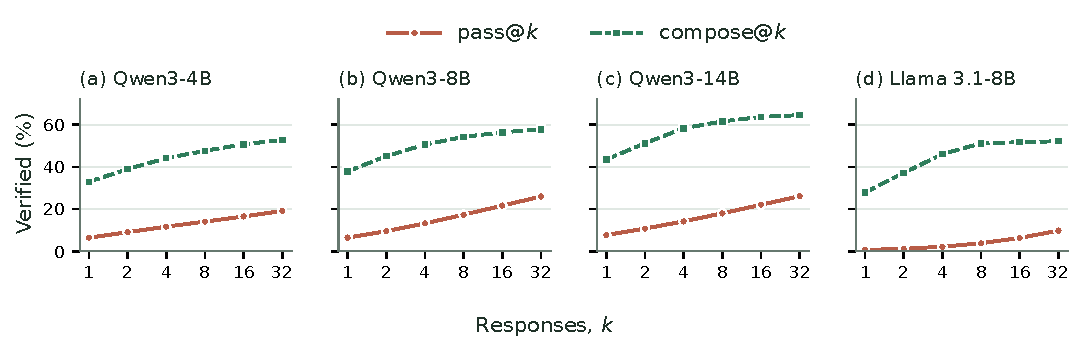
\includegraphics[width=\textwidth]{figures/base_model_probe.pdf}
\caption{pass@\(k\) and compose@\(k\) on the same first \(k\) saved responses.
Composition saturates by \(k{\approx}8\)--\(16\), while pass@\(k\) keeps growing.}
\label{fig:base-model-probe}
\end{figure}

At \(k{=}1\), compose@1 exceeds pass@1 by 26.51--35.84 points across the four
checkpoints.  Both metrics evaluate the first saved response for each task:
pass@1 checks its standalone success, while compose@1 decomposes and filters
its clauses before final verification.  Their difference therefore captures
the benefit of decomposing and filtering one response, before any
cross-response aggregation, subject to prefix sampling variance.

Beyond \(k{=}1\), the curves scale differently.  From 16 to 32 responses,
compose gains at most 2.04 points across the four checkpoints, while pass
gains 2.63--4.34 points.  On all 832 programs, Llama 3.1-8B compose rises
from 27.88\% at \(k{=}1\) to 51.68\% at \(k{=}16\), then only to 52.16\%
at \(k{=}32\), whereas pass rises from 6.30\% to 9.76\% over the latter
interval.  We use these four backbones in the subsequent training experiments.

\begin{insightbox}
\textbf{Finding.}
Under the same model-call and response budget, compose@\(k\) substantially
exceeds pass@\(k\) and saturates earlier.  Compositional utility should
therefore be treated as a first-class optimization target rather than a
by-product of standalone correctness.
\end{insightbox}

% ---------------------------------------------------------------------------
\subsection{RQ2: How Much Do Compositional Inference and Training Improve Verification?}
\label{sec:exp:main}

For each local backbone and training stage, Table~\ref{tab:rcf-paired}
reports pass@\(k\) and compose@\(k\) side by side on all 832 programs at
\(k{=}1,8\); the same summary is included for four reasoning-disabled API
models.  Bare is the untrained checkpoint, and RL applies reinforcement
learning directly to Bare.  Across all four local backbones, SFT raises
compose@1 to 61.30--66.35\%, and subsequent RL adds another 2.40--5.33
percentage points.  Section~\ref{sec:exp:rl} compares the effects of RL from
Bare and SFT initializations.  Full
sampling curves and benchmark-stratum breakdowns are deferred to
Appendix~\ref{app:complete-results}.

\begin{table}[!t]
\centering
\small
\renewcommand{\arraystretch}{0.94}
\setlength{\tabcolsep}{6.0pt}
\begin{tabular}{llrrrr}
\toprule
\rowcolor{algobg}
Backbone & Training & pass@1 & compose@1 & pass@8 & compose@8 \\
\midrule
\multirow{4}{*}{Qwen3-4B}
 & Bare   & 5.27 & 32.93 & 12.50 & 47.60 \\
 & RL     & 1.70 & 48.80 & 4.50 & 62.50 \\
 & SFT    & 40.43 & 62.62 & 59.99 & 76.20 \\
 & SFT+RL (\sam{}) & 33.40 & 66.10 & 49.90 & 74.50 \\
\cmidrule(l{3pt}r{3pt}){1-6}
\multirow{4}{*}{Qwen3-8B}
 & Bare   & 6.43 & 37.86 & 17.33 & 54.21 \\
 & RL     & 6.80 & 57.93 & 16.80 & 70.43 \\
 & SFT    & 41.93 & 63.90 & 61.11 & 76.20 \\
 & SFT+RL (\sam{}) & 30.78 & 69.23 & 47.47 & 76.80 \\
\cmidrule(l{3pt}r{3pt}){1-6}
\multirow{4}{*}{Qwen3-14B}
 & Bare   & 7.67 & 43.51 & 17.97 & 61.54 \\
 & RL     & 10.40 & 65.40 & 18.70 & 72.20 \\
 & SFT    & \textbf{45.66} & 66.35 & \textbf{63.50} & \textbf{78.37} \\
 & SFT+RL (\sam{}) & 40.70 & \textbf{70.80} & 56.80 & 76.80 \\
\cmidrule(l{3pt}r{3pt}){1-6}
\multirow{4}{*}{Llama 3.1-8B}
 & Bare   & 0.61 & 27.88 & 3.81 & 51.20 \\
 & RL     & 4.50 & 46.00 & 10.50 & 56.20 \\
 & SFT    & 39.24 & 61.30 & 56.86 & 73.08 \\
 & SFT+RL (\sam{}) & 33.70 & 63.70 & 49.64 & 72.70 \\
\midrule
\multicolumn{6}{l}{\textit{API models}} \\
GPT-5-nano       & -- & 3.58  & 33.89 & 16.05 & 55.53 \\
GPT-5            & -- & 32.58 & 51.32 & 51.74 & 72.00 \\
Claude Sonnet-4.6 & -- & 36.35 & 56.97 & 44.93 & 66.95 \\
DeepSeek V4-Flash & -- & 28.08 & 51.44 & 48.21 & 74.40 \\
\bottomrule
\end{tabular}
\caption{Main results on all 832 programs (\% verified).  Pass evaluates
complete responses, whereas compose decomposes, pools, and filters the same
response pool.  Bold marks the best value in each column across all rows, including the API
baselines: trained local models lead every column, and \sam{} attains the
best compose@1 (70.80\%).  API rows are evaluated without additional
training.  Complete curves and stratum-level results are in
Appendix~\ref{app:complete-results}.}
\label{tab:rcf-paired}
\end{table}

\begin{insightbox}
\textbf{Finding.}
SFT amortizes multi-response compositional search into a single rollout,
substantially improving exploration efficiency per model call.  RL then
reshapes the exploration distribution using group-relative credit from
negative rejection: one Qwen3-8B SFT+RL rollout reaches 69.23\% compose@1,
surpassing the 57.81\% compose@32 of Bare with 32 rollouts.
\end{insightbox}

% ---------------------------------------------------------------------------
\Needspace{22\baselineskip}
\subsection{RQ3: How Does \sam{} Compare with Specialized Tools?}
\label{sec:exp:tools}

\begin{wrapfigure}{r}{0.50\textwidth}
\vspace{-\intextsep}
\centering
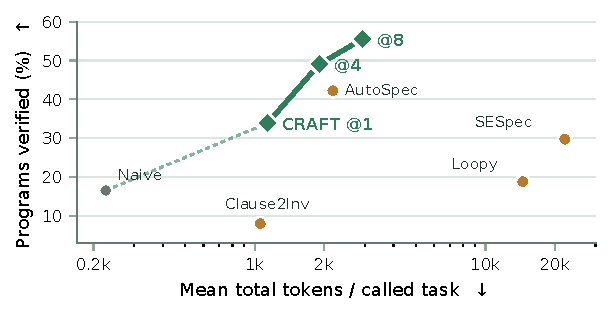
\includegraphics[width=\linewidth]{figures/tool_pareto.pdf}
\captionsetup{font=small}
\caption{Verification rate versus (a) token use and (b) end-to-end time;
Costs are means; upper-left is better.  LLM-based runs use GPT-5-nano
except CRAFT (trained).
Daikon makes no model call and appears only in the time panel.}
\label{fig:tool-pareto}
\end{wrapfigure}
We compare \sam{} with the target-hidden pipelines of AutoSpec, SESpec,
Clause2Inv, Loopy, and Daikon~\citep{wen2024enchanting,yang2026sespec,
cao2025clause2inv,kamath2023finding,daikon}.  The LLM-based baselines and the model-matched \sam{} runs use
GPT-5-nano with reasoning disabled; the trained \sam{} checkpoint is shown
as an additional series.  All outputs face the same untouched
Frama-C/WP judge, and unsupported inputs count as failures among all 832
programs.  Figure~\ref{fig:tool-pareto} compares verification rate against
mean total tokens and end-to-end time under each system's native
orchestration.  In the token panel, all three
GPT-5-nano \sam{} budgets lie on the model-matched Pareto frontier: compose@4 verifies
49.04\% with fewer tokens than AutoSpec, the strongest external baseline in
this reasoning-disabled comparison (42.19\%), while compose@8 reaches
55.53\%.

The trained \sam{} checkpoint reaches 70.31\%, 75.60\%, and 77.28\% at
compose@1, @4, and @8, using 1,348, 2,053, and 2,993 tokens per task,
respectively.  The corresponding mean end-to-end times are 28.2, 33.5,
and 40.9 seconds per task.  At compose@4 and compose@8, the trained
checkpoint has both higher verification rates and lower recorded times than
GPT-5-nano \sam{} (46.40 and 69.99 seconds).  Wall times reflect each
system's serving setup; GPT-5-nano \sam{} times combine archived request
latency with measured prefix filtering and final verification.

We compare systems end to end without matching calls or token
budgets.  Appendix~\ref{app:complete-results} reports accuracy by category,
token use, runtime, and reasoning effort.  The benefit also holds for three
additional API models (Table~\ref{tab:cross-model-main}).

\begin{insightbox}
\textbf{Finding.}
Under target hiding, orchestration efficiency matters as much as proposal
strength.  CRAFT turns independent responses into reusable clauses: all three
GPT-5-nano budgets lie on the model-matched token frontier, and compose@4
simultaneously beats the strongest external baseline in verification rate and
mean tokens.
\end{insightbox}

% ---------------------------------------------------------------------------
\subsection{RQ4: How Does RL Reshape Compositional Exploration Before and After SFT?}
\label{sec:exp:rl}

Prior work suggests that RLVR can reallocate probability toward behaviors
already available to the base model rather than create fundamentally new
reasoning patterns~\citep{yue2025rlcapacity}.  We test this at the level of
compositional utility using matched Bare--RL and SFT--SFT+RL Qwen3-8B pairs
(Figure~\ref{fig:rl-panels}).

From Bare, RL raises compose@1 by 20.07 points and compose@32 by 15.39 while
leaving pass@1 nearly unchanged (6.80\% vs.\ 6.43\%).  One RL rollout reaches
57.93\% compose@1, slightly above the 57.81\% from 32 Bare rollouts.  The
persistent large-\(k\) gain is consistent with sharpening a diffuse long tail,
although the finite sweep cannot establish whether those clauses were already
present.  The same curve-wide improvement holds for the other three backbones
(Table~\ref{tab:rlzero-additional}).

After SFT, RL primarily improves the low-sample regime.  It raises compose@1
from 63.90\% to 69.23\% (+5.33), but the gain contracts to 1.44
points at \(k{=}4\), 0.60 at \(k{=}8\), 0.34 at \(k{=}16\), and 0.47 at
\(k{=}32\).  Equivalently, the gap between compose@1 and compose@32 shrinks
from 14.00 to 9.14 points.  Thus, after SFT has established broad
large-budget coverage, RL mainly moves high-reward candidates into the
small-budget regime rather than materially expanding the solutions recovered
by 32 responses.  Meanwhile, pass@1 and pass@32 fall from
41.93\%/67.98\% to 30.78\%/53.47\%.
This pass reduction is compatible with our inference framework: useful
clauses can still be recovered from a rollout that fails as a standalone
answer, and RL may increase the probability of such rollouts, including ones
with whole-response syntax errors.
The small-\(k\) composition gain holds across all four backbones, all three
strata, and the clause-cap sweep (Tables~\ref{tab:rcf-paired}
and~\ref{tab:rl-complete}; Appendix~\ref{app:clause-cap}).

\begin{insightbox}
\textbf{Finding.}
RL shifts probability mass toward clauses favored by our target-independent
reward, allowing successful compositions to emerge at smaller \(k\).  From
Bare, this improves composition across all measured budgets; after SFT, the
gains concentrate at small \(k\), reducing the sampling budget needed to
recover much of the large-\(k\) performance.
\end{insightbox}

% ---------------------------------------------------------------------------
\subsection{RQ5: How Should Credit Be Assigned for Compositional Inference?}
\label{sec:exp:ablations}

Because targets remain hidden during RL, we use negative coverage of the
pooled survivors as a target-independent surrogate.  From the same Qwen3-8B
Bare initialization, Binary and Whole-rollout use response-level credit,
Clause-decomposed preserves credit for surviving \(V_i\), and Full adds the
group allocation \(w_g\phi_i\) (Equation~\eqref{eq:generation-reward}); all
other settings are fixed.

\begin{figure}[H]
\centering
\begin{minipage}[t]{0.48\textwidth}
\vspace{0pt}
\centering
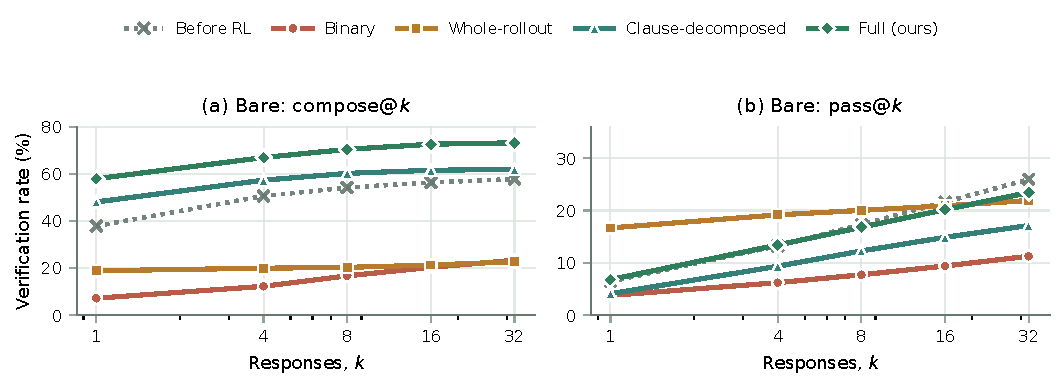
\includegraphics[width=\linewidth]{figures/reward_ablation.pdf}
\caption{Qwen3-8B reward ablations from the Bare initialization.
  Whole-response credit reduces composition; clause and group credit recover
  it.  The matched SFT-initialized controls, where Binary collapses the
  strong SFT composition curve, are in Table~\ref{tab:reward-ablation}.}
\label{fig:reward-ablation}
\end{minipage}\hfill
\begin{minipage}[t]{0.48\textwidth}
\vspace{0pt}
\centering
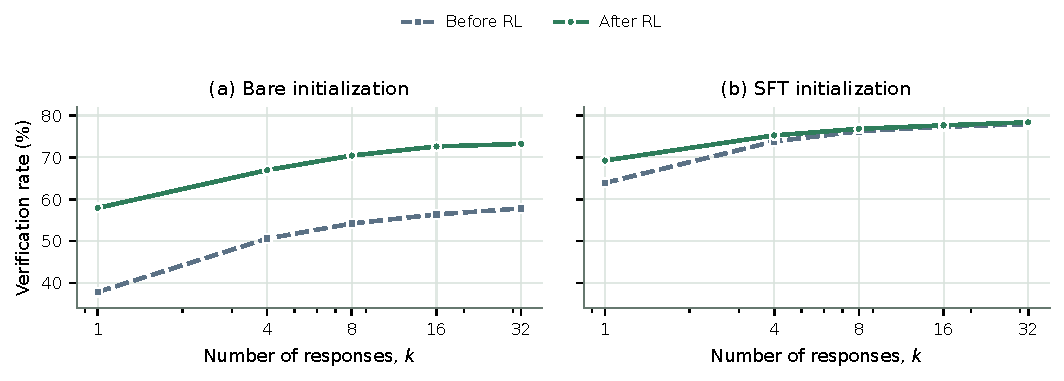
\includegraphics[width=\linewidth]{figures/qwen_rlzero_probe.pdf}
\caption{Matched Qwen3-8B composition curves before and after RL.
  RL improves Bare throughout and raises small-\(k\) composition after SFT
  saturates at large \(k\).}
\label{fig:rl-panels}
\end{minipage}
\end{figure}

Whole-rollout credit raises pass@1 from 6.43\% to 16.67\% yet reduces
compose@32 from 57.81\% to 22.72\%.  This exposes a tension between
single-response correctness and exploration breadth.  Its all-or-nothing
gate withholds credit from every useful surviving clause whenever any clause
in the response is rejected, suppressing partial candidates that pooled
inference can exploit.  Clause-decomposed credit removes the gate and credits
each response for the coverage of its surviving \(V_i\).  Relative to
Whole-rollout, it raises compose@1 from 18.87\% to 48.08\% and compose@32 from
22.72\% to 61.90\%, surpassing Bare by 10.22 and 4.09 points, respectively.

Shapley group credit adds another 9.62--11.30 points across \(k\).  Its
\(1/f(\nu)\) allocation gives more per-response weight to hard or rare
rejections and discounts redundant ones.  This group-relative weighting also
breaks coverage-count ties under GRPO, providing finer advantage signals and
mitigating premature convergence to insufficiently diverse invariants.
In the available SFT-initialized controls, Full improves compose@1 over
Whole-rollout on Qwen3-4B and Llama~3.1-8B, and over Clause-decomposed on
Qwen3-8B; the smaller post-SFT Shapley gain on Qwen3-8B is consistent with lower
within-group redundancy (Tables~\ref{tab:reward-ablation}
and~\ref{tab:clause-cap-structure}).

Structured negatives add 2.0--5.3 compose@\(k\) points over random
perturbations; Appendices~\ref{app:ablation-definitions}
and~\ref{app:coverage-predictiveness} give the full results and predictive
validity analysis.

\begin{insightbox}
\textbf{Finding.}
Training credit should reflect the clauses retained by compositional
inference.  Clause-decomposed credit preserves useful contributions lost
under Whole-rollout's all-or-nothing reward; Shapley allocation further
rewards contributions that reject negatives few other responses can reject.
\end{insightbox}
